% The location law. Numbers: results/PRIMARY_CLAIMS.md, results/CROSS_COHORT.md, results/review2/*.csv, results/round4/
% (generated tables paper/tables/review2_*.tex); full text of the pre-cut version in Supplement S14 and S18.
\section{Results: a location law for ROI masking}\label{sec:law}\label{sec:derm}\label{sec:multi}

\subsection{Controlled sweeps}
With a synthetic ruler whose overlap with the lesion is swept from 0 to 100\% (2,437 ISIC 2018 images, DINOv2 ViT-B/14,
three seeds), ROI masking raises reversed-test AUROC over ERM by $+0.184$ when the ruler lies outside the lesion and
lowers it by $-0.129$ when the ruler lies on it (location interaction $+0.313$ [$+0.258, +0.370$]). At full overlap the
masked model's correlated AUROC exceeds ERM's (0.961 vs 0.937): it uses the ruler \emph{more}. Synthetic calipers on
thyroid nodules and ovarian tumours and synthetic debris on capsule lesions show the same pattern (Fig.~\ref{fig:dose};
all intervals in Supplement~S14).
\ifdupfloats
\begin{figure*}[t]\centering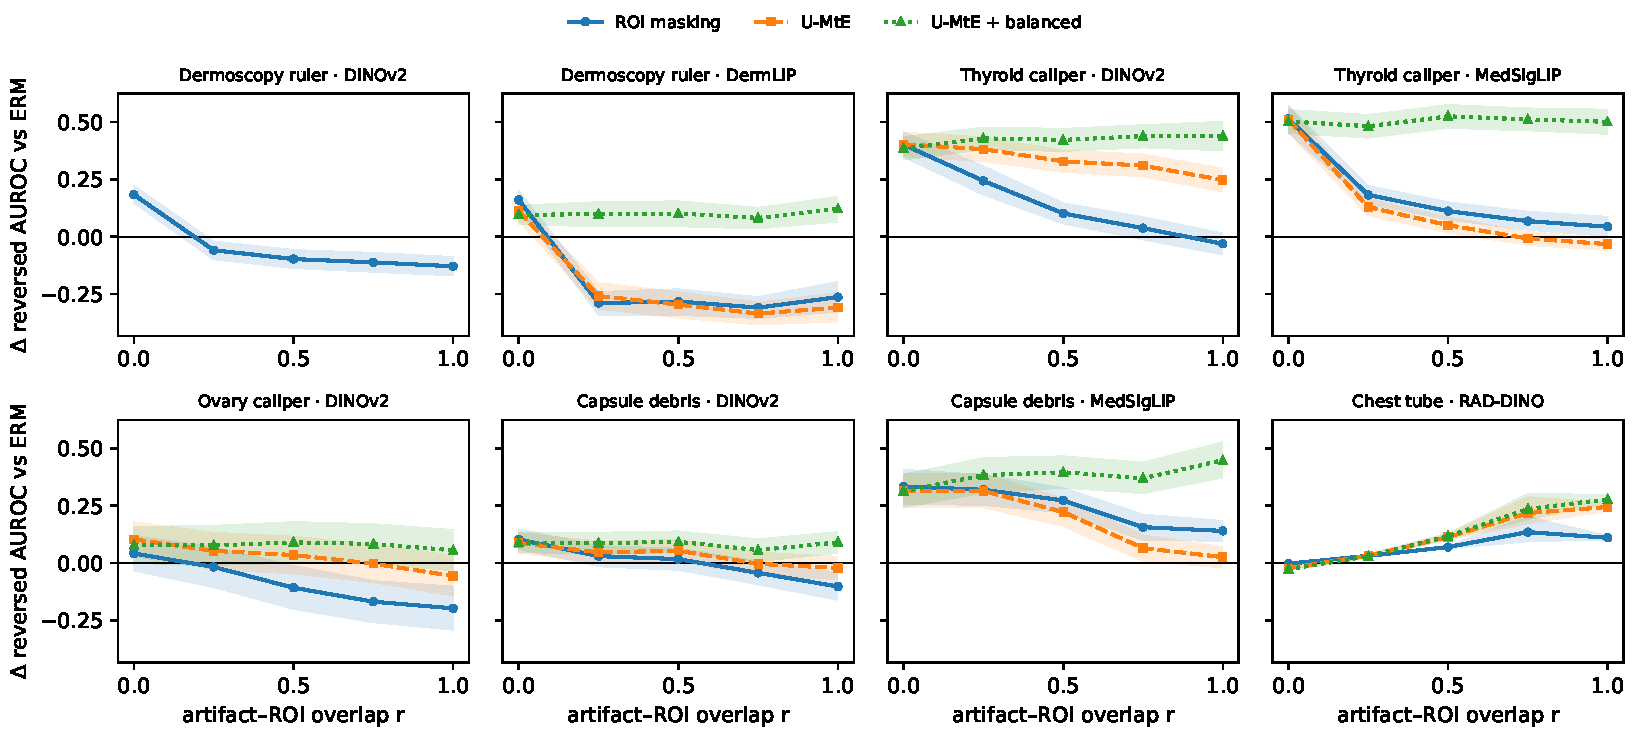
\includegraphics[width=\textwidth]{figures/dose_response.pdf}
\caption{Controlled overlap sweeps: change in reversed-test AUROC versus ERM as the synthetic artifact moves into the
ROI (95\% CIs shaded). ROI masking (blue) declines with overlap in every modality except chest radiography, where the
encoder ignores extra-pulmonary tubes; U-MtE with group balancing (green) is flat. Generated by
\texttt{scripts/make\_figures.py}.}\label{fig:dose}\end{figure*}
\fi

\subsection{Real artifacts in four diseases (pre-registered)}
In the real traps the crossover $[\text{mask}-\text{ERM}]_{\text{Trap B}}-[\text{mask}-\text{ERM}]_{\text{Trap A}}$ is
positive and Holm-significant in all four cohorts, from $+0.147$ for dermoscopic hair to $+0.377$ for capsule debris
(Table~\ref{tab:law}, first column). For hair, masking \emph{harms} when the hair lies on the lesion ($-0.049$
[$-0.083, -0.018$]) and helps when it lies beside it ($+0.098$). For calipers and debris, in-ROI masking still helps,
but far less than out of the ROI (thyroid $+0.109$ versus $+0.348$), and the masked Trap~A model still relies on the
calipers (correlated 0.908 versus reversed 0.398). The registered external test on new patients (ISIC 2020,
patient-disjoint folds, hair masks from a segmenter frozen before any ISIC 2020 image was scored) reproduces the hair
pattern, with harm on the lesion ($-0.064$), gain beside it ($+0.186$) and a crossover of $+0.250$ [$+0.174, +0.327$].
What is universal is therefore the \emph{gap}: masking leaves an in-ROI shortcut largely intact while it removes an
out-of-ROI one. Harm is conditional; it appears when the mask also removes disease context or leaves the artifact a
larger share of what remains (Sec.~\ref{sec:theory}).

\subsection{Location, not image population: transplant and matched traps}\label{sec:transplant}\label{sec:matched}
Trap~A and Trap~B contain different images, and these differ systematically: lesions with hair on them are much larger
(standardised mean difference 2.1), as are thyroid nodules with calipers on them and capsule lesions with debris on
them. We therefore cut real artifact instances---a caliper line with its end crosses, a hair strand, a piece of
debris---from artifact-bearing images and pasted each \emph{inside} or \emph{outside} the ROI of the \emph{same}
artifact-free images, with the same instance, transform and compositing at both locations (pre-registered). Outside
the ROI masking removes the pasted shortcut entirely; inside, the shortcut survives, and the location interaction is
positive in all four cohorts (Table~\ref{tab:law}, third column). A paste-edge control, neutral tissue pasted through the
same masks, gives 52--92\% of the effect: what the transplant isolates is the location of a label-correlated pattern,
not the appearance of a particular artifact; the artifact's own content adds to it significantly for hair and thyroid
calipers only (last column). As an observational check we matched the artifact-bearing images of the two traps 1:1 on
lesion size, artifact amount and acquisition covariates. The crossovers are unchanged (second column), shrink by at most
16\% under a four times stricter calliper, and survive a doubly robust regression on every matching covariate (Holm
$p=0.002$ in each cohort). Matching was infeasible for capsule (19 pairs), where the location evidence rests on the
transplant. Details and balance tables: Supplement~S11.
\begin{table}[t]\centering\small
\caption{The location law under four designs (reversed-test AUROC, DINOv2 ViT-B/14; 95\% crossed seed$\times$image bootstrap CIs, Sec.~\ref{sec:setup}). \emph{Real traps}: crossover $[\text{mask}-\text{ERM}]_{\text{out}}-[\text{mask}-\text{ERM}]_{\text{in}}$ between different artifact-bearing images (rebuilt run). \emph{Matched}: the same after 1:1 propensity matching of the in-ROI and out-of-ROI artifact-bearing images (calliper 0.2 SD; Supplement~S11). \emph{Transplant}: one real artifact instance pasted inside or outside the ROI of the same artifact-free images (location interaction). \emph{Neutral paste}: neutral tissue pasted through the same masks, positions and blending (paste-edge control). Transplant and matching were designed after the real-trap results and registered before their own results; each design is its own Holm family.}\label{tab:law}
\resizebox{\linewidth}{!}{\begin{tabular}{lccccc}\toprule
Cohort & Real traps & Matched & Transplant (artifact) & Neutral paste & Artifact $-$ neutral \\\midrule
ISIC hair & $+0.147$ [$+0.109, +0.185$] & $+0.154$ [$+0.122, +0.187$] & $+0.253$ [$+0.214, +0.293$] & $+0.204$ [$+0.164, +0.244$] & $+0.049$ [$+0.026, +0.072$] \\
Thyroid & $+0.239$ [$+0.196, +0.280$] & $+0.238$ [$+0.186, +0.291$] & $+0.277$ [$+0.256, +0.298$] & $+0.145$ [$+0.130, +0.161$] & $+0.132$ [$+0.116, +0.148$] \\
Ovary & $+0.170$ [$+0.087, +0.253$] & $+0.163$ [$+0.049, +0.274$] & $+0.074$ [$+0.044, +0.104$] & $+0.052$ [$+0.021, +0.084$] & $+0.022$ [$-0.002, +0.048$] \\
Capsule & $+0.377$ [$+0.326, +0.425$]$^\ddagger$ & infeasible$^\dagger$ & $+0.497$ [$+0.427, +0.567$] & $+0.459$ [$+0.383, +0.535$] & $+0.037$ [$-0.017, +0.093$] \\
\bottomrule\end{tabular}}
\par\smallskip{\footnotesize $^\dagger$19 matched pairs in one label, below the pre-registered minimum of 30. $^\ddagger$Descriptive: capsule lesions carrying debris are much larger than those with debris beside them (standardised mean difference 2.6) and matching is infeasible, so this crossover is not by itself evidence about location.}
\end{table}


\subsection{How general the law is}\label{sec:impl}\label{sec:replication}
All four other masking implementations---black fill, blurred background, crop to the lesion box, crop of the masked
image---give a positive crossover in all four cohorts (16 of 16, Holm $p\le0.010$). The two traps are the ends of a
continuous dependence: binned by their real overlap, the mask gain falls with $r$ in every cohort, and for hair it turns
from a gain into a harm near $r=0.4$. The
crossover replicates with MedSigLIP in three cohorts, with a CNN (ConvNeXt-Base) in two, with DINOv2 at three sizes
(nine of nine), with end-to-end fine-tuning in the three cohorts where the network learned the task, and in the
zero-shot scores of vision--language models. The one exception is the dermatology encoder DermLIP: masking costs it
disease signal at both hair locations, and the hair crossover vanishes ($+0.014$ [$-0.037, +0.063$]), as the account of
Sec.~\ref{sec:theory} anticipates. Details: Supplement~S7, S16 and S18.

\subsection{Chest radiography: a boundary case}
A radiograph encoder (RAD-DINO) ignores a synthetic tube outside the lungs, so masking has nothing to remove there. On
real devices (RANZCR-CLiP linked to NIH), lung masking helped at both locations with RAD-DINO; with MedSigLIP, which does
use the out-of-lung tube, the crossover is positive for all four findings. The device contrast is, however, confounded
with other tubes, and real chest drains carry the shortcut through the treated lung. We report
chest radiography as the boundary of the law, not as a fifth confirmation (Supplement~S3).
